\chapter{Contributions in Spatio-Temporal Analysis} % Main chapter title

\label{intro}

\section{Introduction}

As the world becomes interconnected, spatio-temporal data are more ubiquitous and are getting more and more attention.  Moving object (e.g., taxi, bird) trajectories recorded by GPS devices, social event (e.g., microblogs, crime) with location tag and time stamps, and environment monitoring (e.g., remote sensing images) are typical spatio-temporal data that we meet every day\footnote{\url{http://researcher.watson.ibm.com/researcher/view_group.php?id=4152}}. These emerging spatio-temporal data also bring new challenges and opportunities to data mining and machine learning researchers.
This chapter introduces some of the contributions we realized in the past years regarding spatio-temporal data analysis.
It is organized in five parts: the first two sections are more related to works on pattern mining and pattern extraction we developed during the researches conducted in Montpellier. The first section is related to the analysis of Moving Object data realized during the PhD Thesis of Dr. Phan Nhat Hai while the second one introduces my recent experiences related to manage spatial interaction through graph-based approaches.

On the other hand, the third and fourth sections are more focused on classification techniques (supervised and semi-supervised) we conceived in partnerships with other colleagues. The third section involves the work on data stream analysis we developed in collaboration with Prof. Bernhard Pfahringer during my visit at the University of Waikato, New Zealand. The fourth section describes some applications of my research in the field of remote sensing image analysis.

Finally, the fifth section gives a quick overview of my research collaborations in the general field of data mining and machine learning. 

As a general guideline to read this chapter, the contributions we proposed in the different domains are highlighted in bold face.


\section{Moving Object Data: Efficiently extract New, Useful and Non Redundant Trajectory Patterns} 
Techniques able to summarize the behavior of groups of objects moving together are getting more and more attention due to the rapid development of positioning technologies (smartphones, GPS tracking systems, location-based services, etc..) that constantly record and store position information. 

Analyzing data generated from these systems can be useful for:
\begin{itemize}
\item [+] Understanding animal migrations to support public policies in order to preserve biodiversity;
\item [+] Studying and monitor traffic on road networks to better design future transportation systems; 
\item [+] Detecting suspicious or anomaly movement patterns behaviors. 
\end{itemize}

This is why during the PhD Thesis of Phan Nhat Hai, co-supervised with Prof. Pascal Poncelet and Dr. Maguelonne Teisseire we studied, conceived and developed new data mining algorithm to extract and summarize collections of trajectory patterns from moving object dataset.

\subsection{Mine different patterns under a unique approach}
A lot of research was done to analyze such datasets with the goal to extract meaningful patterns~\cite{Han2010} and, at the same time, many algorithms have been proposed such as $CuTS^*$~\cite{Jeung2008} (convoy mining), $ObjectGrowth$~\cite{Li2010} (closed swarm mining), $VG$-$Growth$~\cite{Wang2006} (group pattern mining), etc...
Each of the different proposed methods has its own characteristics and it only extracts one type of pattern. This means that if we want to compare different moving object patterns extracted from the same dataset, we need to re-implement each of the different methods and then run each of the algorithm independently. 

\textbf{This issue was addressed by the {\sc GeT\_Move} approach~\cite{HaiIPT12ep}}. This framework represents the moving object database by a \textit{cluster matrix} in which a row is an object and a column is a cluster of objects at a certain time stamps.
The matrix representation is successively employed to extract frequent closed itemsets from which movement patterns can be mined.

\subsection{Flexible Moving Object Patterns}

One issue shared by all the previous proposed moving object pattern methods regards the way parameters are set. Defining a unique strict threshold, i.e. the maximum time gap between pair of object clusters, without some degree of flexibility can negatively impact the extraction process due to the imposed tight bound.
Another issue that affects many moving object pattern definitions is the constraint related to the object to monitor. Most of the previous approaches~\cite{Han2010} consider that a pattern is defined over the same set of objects but, if we for instance consider animal migration, different objects can join (or leave) a group of objects that is moving towards a certain direction. Also in this case the data mining method needs to model some degrees of flexibility to manage such a situation.

As the data can contain noise or the user has approximate knowledge about the data itself, allowing to soften certain constraints or manage graduality in the objects that belong to a pattern can alleviate such problems.  

\textbf{In~\cite{HaiIPT12adma} we design and develop a fuzzy pattern mining approach to soften the time gap constraint in the field of moving object data mining.}  This pattern definition allows the user to define an interval time gap (minimum/maximum) and fuzzy logic operators are introduced to retrieve patterns that match the fuzzy constraints. From an algorithm point of view, we still exploit an itemset-based representation so that {\sc GeT\_Move} can be employed to gather all the fuzzy moving object patterns.

\textbf{The issue related to analyze and extract object trajectories in which individuals can join (or leave) the backbone of the pattern is addressed by~\cite{HaiIPT12}}. The proposed algorithm manages gradual moving object patterns which satisfy the graduality constraint during at least $min_t$ timestamps. As state before, the graduality constraint allows the number of objects to increase (or decrease) while the set of remaining objects shared should be the same among the clusters.


\subsection{Mining Representative Moving Object Patterns} 
Most of the researches in moving object mining are focused to extract specific trajectory patterns that differ in their characteristics with the goal to capture various aspects of the data~\cite{Jeung2008,Li2010,Wang2006,HaiIPT12}. All these methods extract thousand of patterns resulting in a huge amount of redundant knowledge that is difficult to exploit. Spatio-Temporal databases involve complex information. Due to this complexity, studying a spatio-temporal database by employing only a single type of pattern is not enough to depict an informative picture of the data.  

\textbf{Motivated by these issues, we develop a Minimum Description Length (MDL)-based approach that compress spatio-temporal data leveraging different kinds of moving object patterns~\cite{HaiIPT13}.} 


The proposed approach introduces a way to evaluate to which extent each extracted pattern is useful and not redundant to summarize  the original spatio-temporal dataset. The MDL criterion allows to rank the set of heterogeneous patterns selecting only those that best compress the data and discarding all the useless ones.






\section{Spatial Interaction: One more piece of the puzzle}

During the last years, I moved more and more my attention towards the analysis of remote sensing data. Such source of information still belongs to the category of spatio-temporal data but, differently from the information I worked on before, it has some peculiarities: i) the spatial dimension plays a role at least as important as the temporal aspect; ii) data are mainly represented through images; iii) in most cases images are multi-bands (or hyperspectral) and they can be enriched by additional spatial information (Digital Terrain Model, etc.). 
Classical data mining and machine learning approaches cannot be directly applied on such data without an important pre-processing and transformation step and, such operation needs to be adapted to the particular task we would deal with. 

In the field of spatio-temporal data analysis, modeling the data via graph-based representation can be beneficial to analyze information from both spatial~\cite{TuiaMGM13} and temporal~\cite{BringmannBBG10} point of views. From a spatial point of view, the graph structure can supply many information about how the objects of the database are arranged while, from a temporal perspective, explicitly state the links (or relationships) among objects in a graph can help to describe and/or simulate a temporal process.

Graphs, in computer science, are an ubiquitous structure that can be easily employed to model real world information. This tool is particularly suitable to represent interactions between data~\cite{Aggarwal:2010:MMG:1738952}. Examples of graph data are social networks, gene-gene interaction networks, linked open data, document networks, knowledge graphs, etc...
On the other hand, the flexibility of such a structure also allows to model data that does not naturally fit the network paradigm. The graph representation helps to highlight the interaction among the objects of the data and this interaction can be leveraged by specialized data mining and machine learning methods. For example, a textual collection can be represented as a graph where documents are nodes and a link exists between two nodes (documents) if their similarities is above a certain threshold~\cite{RomeoIT15}. Another similar example is supplied by the analysis of remote sensing images. 
After a first pre-processing segmentation step, the image segments can be represented by nodes and a link exists between two nodes if their corresponding segments spatially overlaps~\cite{GuttlerACINPT14} or they have similar spectral signature~\cite{Guttler16}.



\subsection{Understanding Temporal Evolutions}
During the last period I gave more and more attention, as an application domain, to the analysis of Remote Sensing data.
In particular, thanks to the collaboration with experts in remote sensing analysis, we developed new data mining and machine learning approaches especially tailored for this kind of data.
Recently, during the post-doctoral period of Dr. Fabio Guttler, we have started to employ graph-based analysis to model and describe temporal evolutions from time series of satellite images~\cite{GuttlerACINPT14,GuttlerITNP14}. A sketch of the process is illustrated in Figure~\ref{evol_bpa}. 

Given a time series of satellite images the method performs the following steps: i) segments all the images by collecting together all the segments; ii) among the segment set, it chooses a set of reference objects maximizing the covering of the study area and minimizing the overlapping between the chosen reference objects. A reference object can come from any image of the time series; iii) For each reference object, it builds a DAG (Directed Acyclic Graph) that connects all the segments that intersect the reference object over all the images of the time series. The obtained DAG is a $K$-partite graph where $K$ is equal to the number of images in the time series~\cite{GuttlerACINPT14}. A direct edge exists in the DAG if the segment at level $K-1$ (segment of the image $K-1$) spatially intersects the segment at level $K$ (segment of the image $K$). Figure~\ref{evol_graph} shows an example of an evolution graph (DAG) with the corresponding segments ordered by time stamps. 

\begin{figure}[!ht]
\begin{center}
	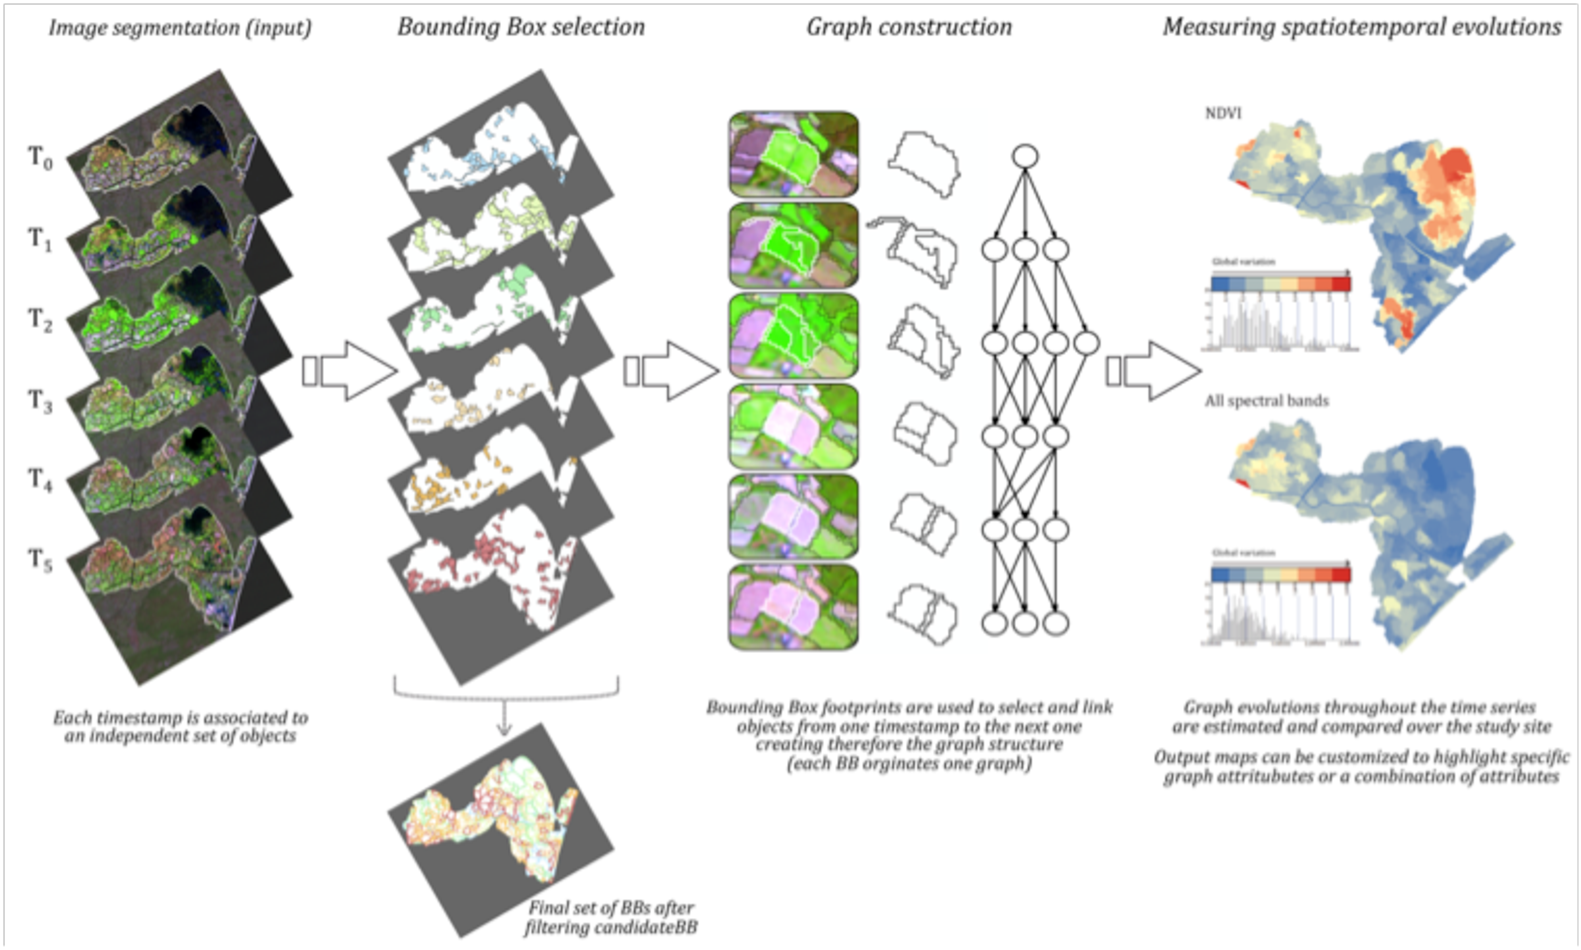
\includegraphics[width=0.90\textwidth]{Figures/evol_bpa.pdf}
\end{center}
\caption{\label{evol_bpa} (Guttler et al. - to appear) The framework to extract evolution graphs from a time series of Remote Sensing Satellite Images.}
\end{figure}

 

\begin{figure}[!ht]
\begin{center}
	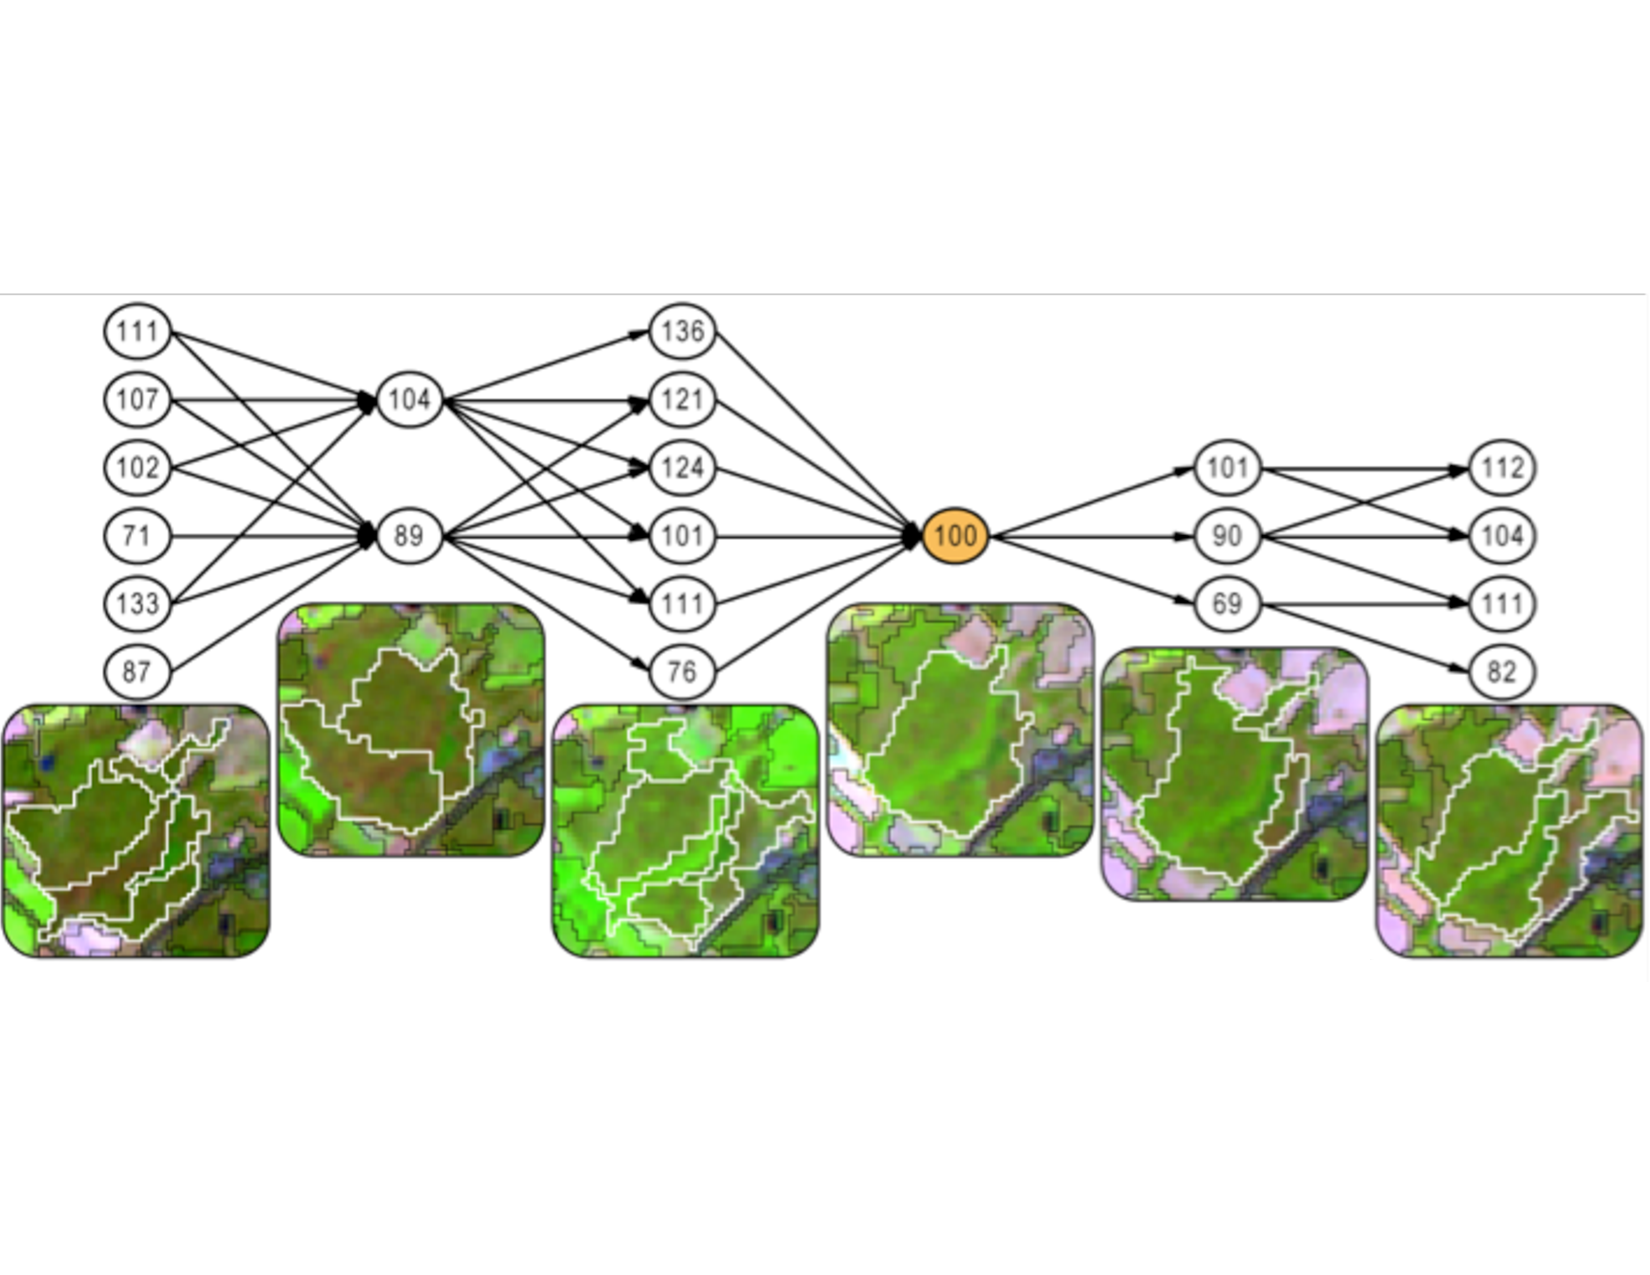
\includegraphics[width=0.70\textwidth]{Figures/evolution_graph.pdf}
\end{center}
\caption{\label{evol_graph} (Guttler et al. - to appear) An example of evolution graphs ($K$-partite DAG) from a time series of six images.}
\end{figure}


A graph can be easily exploited to describe the evolution of a zone. Given a study area (represented by a time series of satellite images), a collection of evolution graphs can be extracted. Such a set of graphs can describe the different phenomena present in the data.
Most of the previous proposed methods mainly contemplate an analysis at pixel level for a reduced number of images (two or three)~\cite{Hussaina13} while the novelty of our proposal lies in the use of objects instead of pixels to describe spatio-temporal evolutions.


\subsection{Manage Rich Relational Structure}
Simple graph structures, sometimes, are not enough to well describe the richness of real world data.
Nowadays many types of data exhibit complex relational structures where additional information in the form of multiple edges between nodes exist. Such kinds of network structures can be defined as multigraphs or multilayer graphs~\cite{PapalexakisAI13, RedondoSIZP15, Ingalalli16, Bourqui16}. They allow different types of edges in order to represent different types of relations between vertices~\cite{BodenGHS12,TangWL12,BonchiGGU14,JinHWRX10}.
Many real world scenarios can be modeled as multigraphs. For instance, by considering different social networks spanning over the same set of people, but with different life aspects (e.g. social relationships such as Facebook, Twitter, LinkedIn, etc.), we can get as many edge types as different aspects. In biology, protein-protein interaction multigraphs can be created considering the pairs of proteins that have direct interaction, physical association or they are co-localised~\cite{BonchiGGU14}. In addition to these examples, Resource Description Framework (RDF) graphs can be naturally represented as multigraphs where the same subject/object node pair is connected by different predicates (properties) that describe different types of relationships~\cite{LibkinRV13}.

\textbf{Recently, I focused my attention to the study of such particular structures~\cite{PapalexakisAI13, RedondoSIZP15, Ingalalli16, Bourqui16} not only because multigraphs can model a wide range of application scenarios but, they can be extremely useful to model, mining and analyze spatio-temporal data. More in detail, in the context of the PhD Thesis of Mr. Vijay Ingalalli, we have designed and developed efficient methods to deal with the problem of subMultigraph iso and homomorphism~\cite{Ingalalli15,Ingalalli16}.} Both problems are known to be NP-Complete and, to some extent, the homomorphism problem is more general than the isomorphism one. %Due to the complexity of the problems, our solutions are based on heuristics that practically show more than reasonable performances. 

In the case of the multigraph structure the sub isomorphism test needs to take into account the topological structure but also the containment relationships between the edge set linking a pair of nodes. An example is given in Figure~\ref{fig:SubMultiGraphIso}. In this example, we can observe two graphs: $G1$ and $G2$. The table in Figure~\ref{fig:SubMultiGraphIso} reports the set of embeddings of graph $G1$ in graph $G2$ with the corresponding mapping. If we consider the embedding $Emb$ 1 the edge ($u1$,$u2$) of $G1$ matches the edge ($v2$,$v3$) because the red edge between ($u1$,$u2$) is contained among the edges (red, green) between ($v2$,$v3$). The same consideration applies for the $Emb$ 2. 


\begin{figure}[!ht]
\begin{center}
	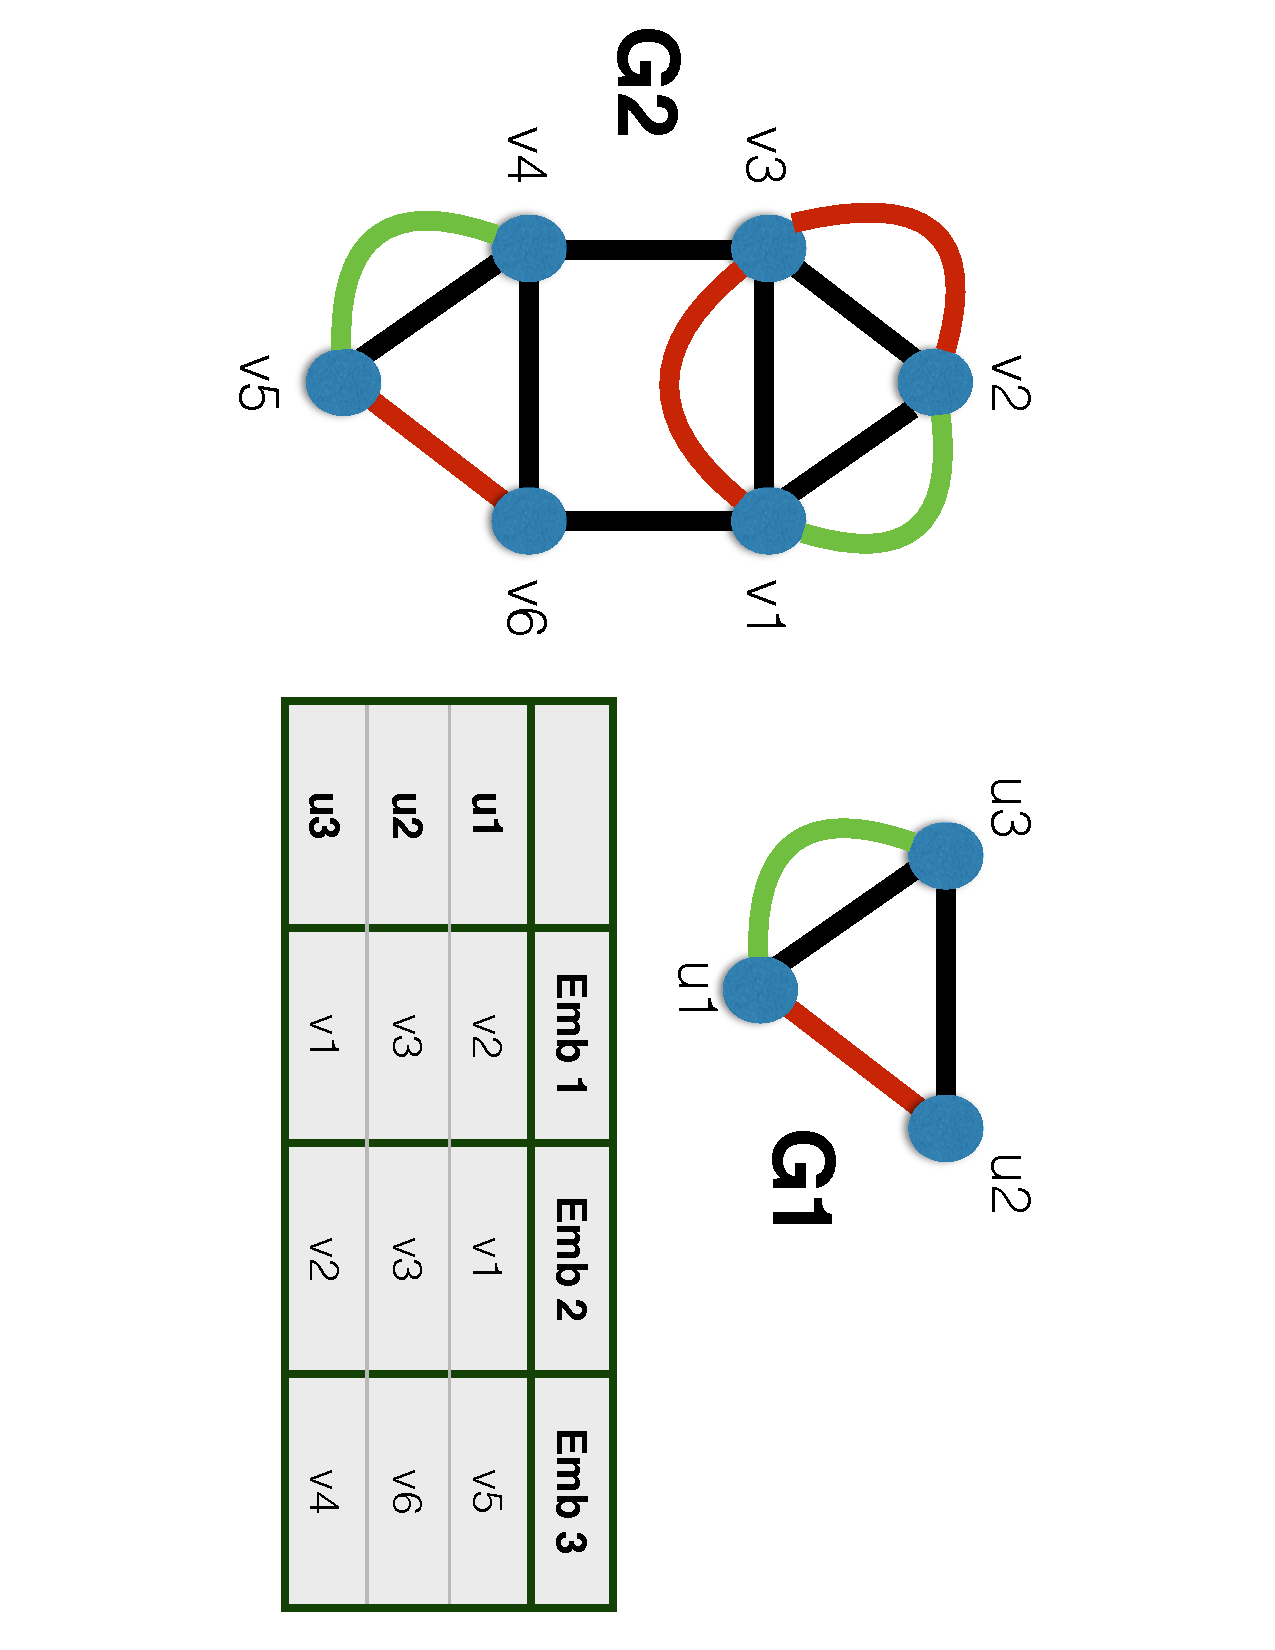
\includegraphics[angle=90,width=0.70\textwidth]{Figures/iso_multi.pdf}
\end{center}
\caption{Sub Isomorphism on Multigraph: Embeddings of $G1$ in $G2$. The table list the possible matching between nodes in $G1$ and vertex in $G2$.  \label{fig:SubMultiGraphIso}}
\end{figure}

Efficiently performing subgraph matching is useful for image analysis~\cite{GautamaBTP07} as it can be used as a flexible query mechanism to answer spatial queries. The original image can be represented by a graph structure and the goal is to detect and retrieve all the portions of the images that match a certain geospatial pattern. 

\section{Remote Sensing Classification: Application to Satellite Images}

%\subsection{Classification}
Remote sensing images are an useful source of information to monitor spatio-temporal phenonmena~\cite{XueSQDW15}.
The increasing number of projects and researches about remote sensing supplies huge amounts of data that are produced almost every day. For instance, the SENTINEL project\footnote{\url{http://www.satsentinel.org/}} promises to capture high-resolution images every five/ten days producing a huge volume of images to process. Studying and developing suitable machine learning and data mining techniques to efficiently manage such kinds of data can be crucial for different purposes such as: food monitoring in remote regions, climate change understanding, land cover and land use classification, complex landscape description~\cite{Mueller-Warrant15,TsangJ10}.


\subsection{Combine Active and Transductive Learning}
Data labels are usually difficult and expensive to obtain. Standard classification techniques heavily rely on the hypothesis that a big quantity of labeled examples (training set) is available to build a predictive model. Considering the remote sensing domain the label acquisition constitutes a time and effort consuming task for the expert~\cite{DemirMB14}. 
Classical supervised inductive classification approaches (i.e. SVM, Naive Bayes, Random Forest, etc.) require many labeled data to train the model. Also, they assume that training and test data are not available at the same time since the model they have learnt needs to be general enough  to classify new unseen examples available in a near future~\cite{0097035}. However, in the case of remote sensing image classification, training examples are limited and all the examples (training and test) are available at the same time. Most of the time, a predictive model is learnt on a portion of the image and it is successively employed to classify the rest of the same image.
\textbf{To tackle these two characteristics in land cover classification: i) data labels acquisition and ii) training and test data available at the same times, we propose in~\cite{Guttler16} a new active/transductive learning framework to cope with object-based remote sensing classification.}
Transductive learning~\cite{SousaRB13} belongs to the family of semi-supervised approaches. The goal of this kind of methods is to propagate information from the labeled data to the unlabeled one leveraging the availability of training and test data at the same time. These kinds of techniques offer an effective approach to supply contextual classification of unlabeled ones by using a relatively small set of labeled examples.
To deal with both label scarcity and quality of training set, we couple the transductive strategy with active learning with the goal to improve accuracy performance and supply a valid alternative to standard classification techniques usually employed in remote sensing domain such as Support Vector Machines and Random Forest~\cite{HuangZ13}.

\subsection{Time Series}

Although data from satellite images are very useful for monitoring land surface, the large quantity of spatio-spectro-temporal measurements stored by the instruments limits the usefulness as sources of information. In recent years, research on spatio-temporal databases has consequently increased alongside research on mining such data~\cite{BogornyS10}. 
\textbf{In~\cite{PitarchIVBLPST15} we deal with the classification of remote sensing time series data with the purpose to characterize land use in the northern fringe of sub-Saharan Africa}. 
In this work we put a major stress on the temporal dimension.
More in detail, we developed a data mining methodology to extract multidimensional sequential patterns to characterize temporal behaviors. In the same spirit as~\cite{MeoBI12}, we used the extracted multidimensional sequences to build an associative classifier, and show how the patterns help to discriminate among the classes. We evaluated our technique using a real-world dataset with the purpose to automatically recognize the land use of a certain area.

\section{Data Stream Classification: Deciding when update the model} 

Many real world applications continuously generate huge amounts of data, such as web logs, sensor networks, business transactions, etc. 
These {\em data streams}~\cite{aggarwal2007book}, due to the big volumes of information they contain, pose serious issues for the research community in order to extract useful and up-to-date knowledge in real-time. Due to its intrinsic temporal dimension, the information available in data streams can change and evolve over time. 
More precisely, this phenomenon impacts on the performance of any supervised (or unsupervised) model learnt over these evolving data: previous models may not be suitable for newly incoming data~\cite{aggarwal2007book}. Therefore we need to adapt models both quickly and accurately.


\subsection{Active Learning}
Learning predictive models on streaming data implies having continuous access to the true values of the target variable (the true class labels) of every incoming example.  This labeling phase is usually an expensive and tedious task for human experts. 
Consider, for example, textual news arriving as a data stream. The goal is to predict if a news item will be interesting for a given user at a given time. The interests and preferences of the user may change over time.
To obtain training data, news items need to be labeled as interesting or not.
This requires human labor, which is time consuming and costly. 
For instance, Amazon Mechanical Turk\footnote{https://www.mturk.com} offers a marketplace for intelligent human labeling.
Labeling can also be costly or practically unfeasible because it may require expensive, intrusive or destructive laboratory tests. 
The labeling problem in standard machine learning scenario is well known~\cite{TongK00} and it is mainly addressed through techniques that guide the construction of the training set by the needs of the predictive models. Such kinds of techniques belong to the family of active learning~\cite{FuZL13}.
\textbf{To address this important issue in the context of data streams, during the period spent at the University of Waikato, in collaboration with Prof. Bernhard Pfahringer and other colleagues, we developed new active learning strategies especially tailored to efficiently learning predictive models on evolving data streams~\cite{IencoBZP13,IencoZP14}.} All the proposals we developed are based on the idea that important instances to sample lie in a high density partition of the data space. In~\cite{IencoBZP13} we instantiate this idea by exploiting clustering approaches in order to estimate the density around each point while in~\cite{IencoZP14} we estimate the density in an online manner, a sliding window mechanism allows to quantify the importance of a point considering the density of its nearest neighbors. 

\subsection{Categorical Change Detection}
Due to its intrinsic temporal dimension, the information available in data streams changes and evolves over time. 
In particular, different types of changes may happen in the stream. For instance, classes or concepts that can be underrepresented during a short period can become overrepresented after a longer period. 
Most of the time, a common assumption made by many research works is to consider only the aposteriori probability of the class given the data~\cite{Gama04,BifetRPHZ13}. This formulation of the change detection task does not exploit information coming from the underlying data distribution. Another issue is that, in real world applications, data is heterogeneous and often can be represented over set of categorical attributes as well as numerical ones.
In the last decade, lots of approaches have been defined to monitor classification accuracy as evidence or an indication for change in streams of numerical data~\cite{BifetRPHZ13} but, few approaches dealing with the same problem for categorical evolving data streams~\cite{CaoH13}. \textbf{In~\cite{IencoBPP14}, we tackle this issue and we propose a new change detection approach devoted to retrieve changes in categorical evolving data streams.}
The proposed approach detects and highlights changes in categorical data streams in a fully unsupervised setting. 
It works in the batch scenario: when a new batch arrives, firstly the algorithm summarizes the block through some statistics and successively performs a statistical test to evaluate if a change happens in the data distribution, or not.
The developed algorithm supplies a segmentation approach that can also work with other statistics. This means that it can be coupled with any other measure we want to monitor.



\section{Other Research Activities in Data Science} 
During the last years, I devoted a major part of my researches to analyze spatio-temporal data but, in order to enrich my methodological background in the field of data mining and machine learning, we studied, conceived and developed, in partnerships with other colleagues, approaches to manage different kind of data such as textual, categorical and linked open data. The motivation related to these researches is that, a methodology we can apply on textual data (i.e. supervised classification, clustering algorithm, etc.) can be adapted and reused, to some extent, for spatio-temporal data analysis.
As example, in the field of multilingual document classification we experimented and apply transductive based methods~\cite{RomeoIT15} and, successively, we extend and adapt the same strategy to perform active transductive classification in the context of object oriented Remote Sensing analysis~\cite{Guttler16}. Study and design general data mining and machine learning methods allows me acquire a good knowledge on how customize each of such strategy w.r.t. the particular domain to investigate. 

\subsection{Clustering and Co-Clustering Unstructured data}
Most of the techniques developed during my PhD training were devoted to unsupervised analysis and in particular to cluster data. During the last years, we continue, with the colleagues I am working with, to conceive and propose new clustering techniques . Most of the proposed techniques were devoted to analyse textual information. 

The choice of this source of information as type of data is due to its ubiquitous nature and to the fact that it is generally not so difficult to retrieve annotated document collections. The availability of labeled data facilitates the evaluation of the different methods. 

\textbf{As a direct extension of my PhD work, we have developed new co-clustering techniques for dynamic textual sources of information~\cite{PensaIM14} and co-clustering techniques for heterogeneous data~\cite{IencoRPM13}.}
In the domain of dynamic textual data we developed approaches able to incrementally cluster streams of text supplying a hierarchical organisation of such documents. The hierarchical organisation allows to easily explore and browse the content of the evolving document collections.
In the same period, we also focused our attention to develop clustering methods that allow the grouping of entities that have an heterogeneous representation. For instance, in~\cite{IencoRPM13} we show how entities that can be described, at the same time, by both visual (images) and textual (captions) information can be jointly analysed in an unsupervised way.

Data heterogeneity is an important characteristic of modern sources of information. The same information can be described by different representations or by different media. An example of such heterogeneity, in the field of text analysis, is supplied by multilingual document collections~\cite{RomeoTI14} in which the same information can be available in different languages. 
\textbf{During the co-supervision (with Dr. Andrea Tagarelli) of the PhD Thesis of Dr. Salvatore Romeo, we designed and developed on unsupervised and semi-supervised machine learning framework to analyse multilingual document collections~\cite{RomeoTI14,RomeoIT15}. }
To tackle the issue of language heterogeneity, we leverage knowledge-based resources~\cite{NavigliP10} to obtain a common representation for collection of multilingual documents. Once the new representation was obtained, we have developed new data mining techniques to automatically categorise multilingual textual information~\cite{RomeoTI14}. In the context of multilingual textual clustering we modeled the documents by a tensor representation and we successively factorized such tensor to find a low dimensional embedding of the original data that helps the clustering process. In the context of semi-supervised textual categorization~\cite{RomeoIT15} we have employed a graph-based transductive learner to propagate label information from labeled documents (written in a certain language) to unlabaled ones (written in the same or another language). The propagation process supplies the final classification result. 


\subsection{Semi-Supervised Learning in Categorical Data}

Supervised and Unsupervised settings, from a machine learning perspective, are two extreme cases in which, from one side, we have labels for all the training data and, from the other side, we do not have class information for any of the objects we would analyse. In many real world tasks the situation is less strict and, we can have situation in which only a portion of the data has associated labels. We can image a scenario in which we need to classify home pages vs. non home pages. In this context we have a good knowledge about what is an home page but, strictly define what is not an home page can be difficult. Examples of such scenario are semi-supervised anomaly detection~\cite{ChandolaBK09} and positive and unlabeled learning~\cite{LiGE11}.
Due to the variety of contexts in which semi-supervised analysis can appear, this is also valid in the context of remote sensing image analysis~\cite{Guttler16}.
\textbf{More in detail, in~\cite{iencoTNNLS16} we recently proposed a semi-supervised anomaly detection for categorical data where a model is learnt on "normal" data and then the learnt model is employed to rank anomalies entities. For the problem of positive and unlabeled learning, we propose in~\cite{iencoNeuro16} an approach that firstly computes a model for the positive class, secondly a set of representative examples for the negative class is detected and finally a discriminative model is built considering both positive and negative instances.}

The peculiarity of the strategies we proposed is related to the data they manage: all the examples are represented by only categorical variables (any numerical variable can be discretized to obtain a categorical one). The problem to employ distance-based machine learning methods on categorical dataset is related to the notion of distance measure~\cite{ChandolaBK09}. Unlike numerical attributes, it is difficult to define a distance between pairs of values of a categorical attribute, since the values are not ordered. This underlines the fact that adapt distance-based machine learning methods to manage categorical information is challenging.

\section{Conclusion}
This chapter resumes the major researches I developed in the last years in collaborations with my colleagues. 
Most of the themes we addressed are related to the design of general data mining and machine learning techniques that can be applied on spatio-temporal or complex data. Each of the addressed topic can supply ideas or hints for possible follow-ups. For instance, regarding the study of moving object data, a  deeper investigation can be made on how moving object patterns can be summarized and how such results can be presented. 
In the data stream scenario, a possible point to address could be the study of how coupling active learning and semi-supervised learning or how unsupervised change detection techniques can help unsupervised learning (such as clustering) to extract useful information from evolving data.
Any of the previous macro topics can supply ideas and point out possible research tracks in the domain of spatio-temporal, textual or categorical data analysis. 

In the next chapter I will try to sketch some of the research directions I would investigate that are deeply connected to my current research in spatio-temporal data analysis.

%\subsection{Managing and Model Linked Open Data}




%%%%%%%%%%%



